\section{Boundary Conditions (BC)}
\subsection{Interface Conditions}
\begin{minipage}[rt]{8cm}
	\begin{tabular}{ll}
		\(\displaystyle \left(\vec{D}_1 - \vec{D}_2\right) \cdot \vec{n} = \rho_S\) & \(\displaystyle \rightarrow D_{n1} = D_{n2} \textrm{ if } \rho_S = 0\)\\
		\(\displaystyle\left(\vec{B}_1 - \vec{B}_2\right) \cdot \vec{n} = 0 \) & \(\displaystyle \rightarrow B_{n1} = B_{n2}\)\\
		\(\displaystyle\left(\vec{H}_2 - \vec{H}_1\right) \times \vec{n} =\vec{J}_S \) & \(\displaystyle \rightarrow H_{t1} = H_{t2} \textrm{ if } \vec{J}_S = 0\) \\
		\(\displaystyle\left(\vec{E}_2 - \vec{E}_1\right) \times \vec{n} = 0 \) & \(\displaystyle \rightarrow E_{t1} = E_{t2} \)\\
	\end{tabular}
\end{minipage}
\begin{minipage}[lt]{11cm}
	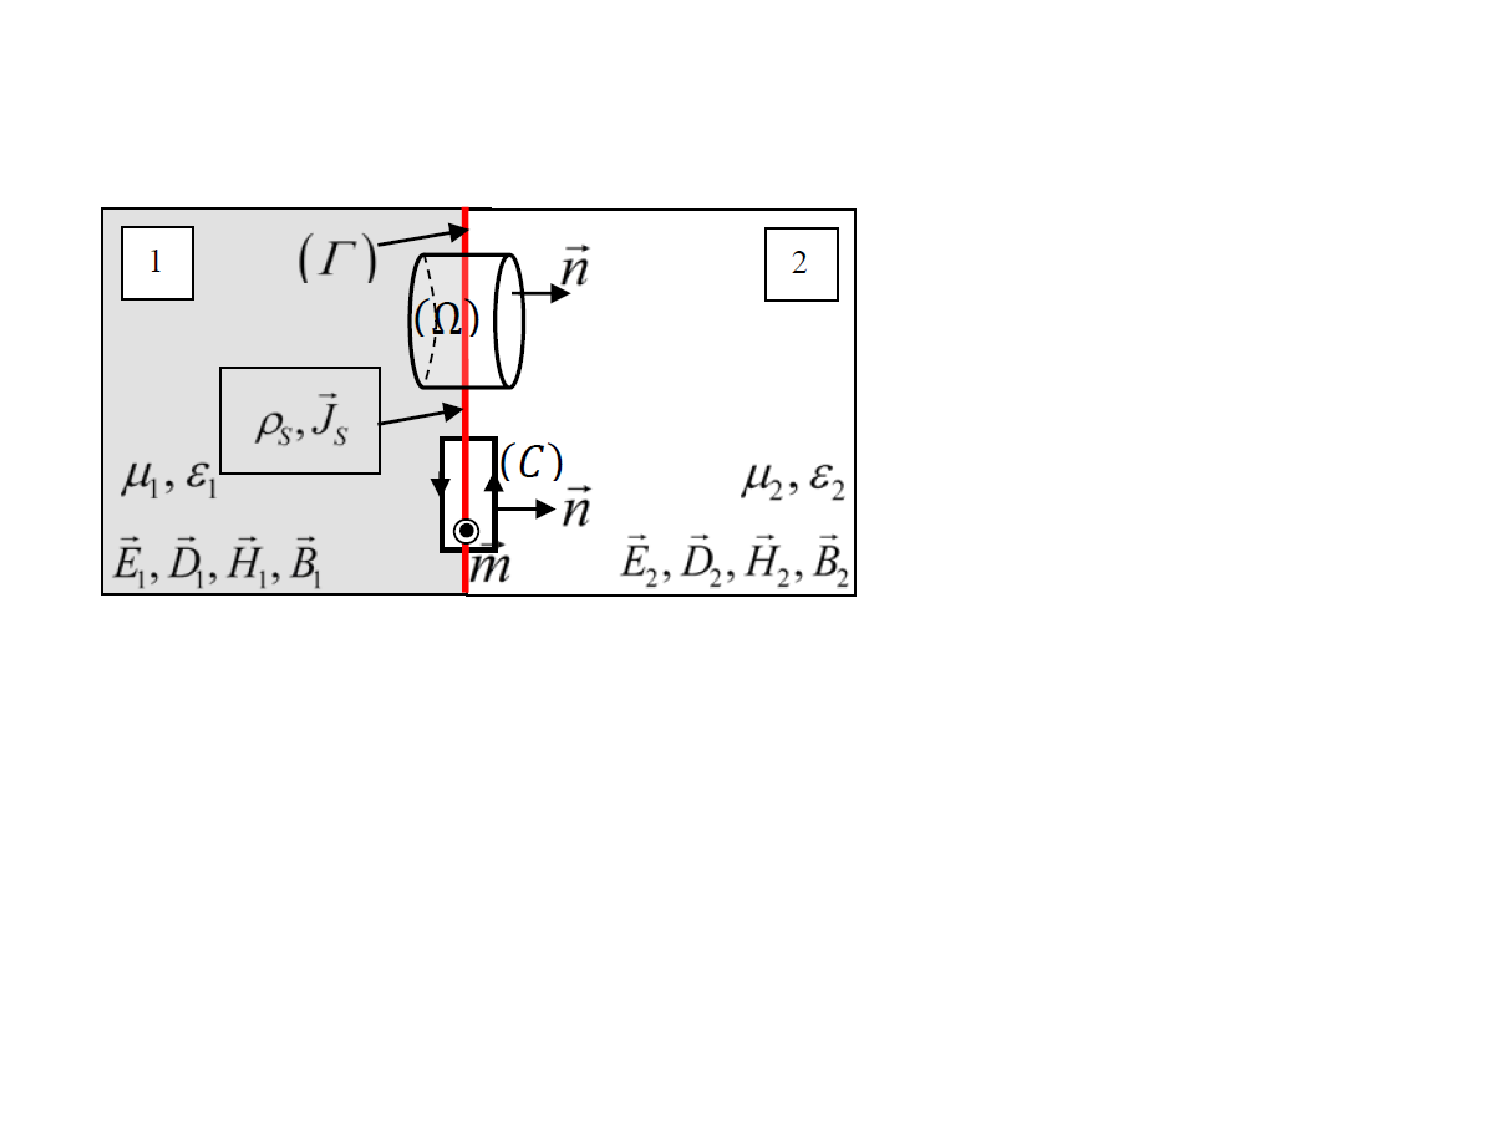
\includegraphics[width=.6\textwidth]{./images/InterfaceConditions.pdf}\\
\end{minipage}
The above interface conditions show the field behavior over the border between two different materials. \newline
The normal flux density continuity conditions can be derived by integrating Equations (\ref{eq:MaxwellInt1}) and (\ref{eq:MaxwellInt2}) over the cylinder $\Omega$ depicted above. (valid as long as there is no charge $\rho_s$ in the boundary) \newline
The tangential field continuity conditions can be proven by integrating Equations (\ref{eq:MaxwellInt3}) and (\ref{eq:MaxwellInt4}) along the contour $C$ shown above. (valid as long as there are no currentss $J_s$ in the boundary)